\documentclass{beamer}

\usetheme{Montpellier}
\usepackage{tikz}

\definecolor{beamer@blendedblue}{rgb}{0.3,0.5,0.6}

\setbeamercolor{normal text}{fg=black, bg=white}
\setbeamercolor{alerted text}{fg=red}
\setbeamercolor{example text}{fg=green!50!blue}

\title{Virtual Reality for Sensor Data Analysis}
\subtitle{SW-Projekt SS 2017 Gruppe 5.1}
\author{Gero Birkh\"olzer \and Johannes Blank \and Alexej Gluschkow \\ \and Fabian Klopfer \and Lisa-Maria Mayer}
\date{Zwischenpr\"asentation am 12. Juni 2017}



\addtobeamertemplate{frametitle}{}{%
\begin{tikzpicture}[remember picture,overlay]
\node[anchor=north east,yshift=2pt] at (current page.north east) {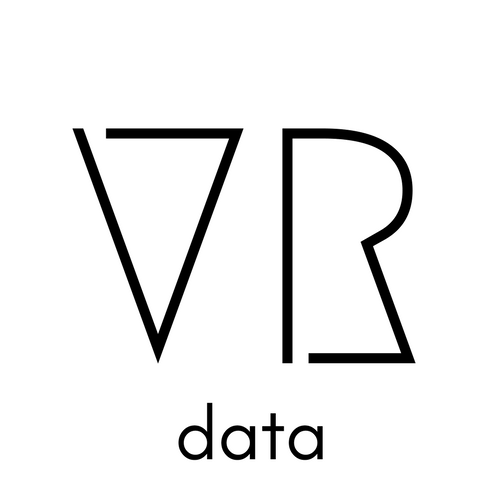
\includegraphics[height=0.8cm]{logo.png}};
\end{tikzpicture}}


\begin{document}


\frame{\titlepage}



\begin{frame}
  \frametitle{Inhalt}
  \tableofcontents%[hideallsubsections]
\end{frame}


\section{Einleitung}

\subsection{Aufgabenstellung}

\begin{frame}
\frametitle{Einleitung}
\framesubtitle{Aufgabenstellung}
\begin{itemize}
	\item Visualisierung von mindestens einem Sensorwert (z.B. Temperatur) in Abhängigkeit von seiner Position.
	\item Verschiedene Visualisierungsmöglichkeiten der Sensordaten.
	\item Visualisierung in einer fertigen 3D Umgebung, basierend auf der Originalumgebung.
\end{itemize}
\end{frame}

\subsection{Idee} %Requirements

\begin{frame}
\frametitle{Einleitung}
\framesubtitle{Idee}
\begin{itemize}
	\item Aufzeichnen von Daten mit der App.
  \item Positions tracking \"uber das smart phone.
  \item Anzeigen dieser Daten in der WebVR Umgebung.
\end{itemize}
\end{frame}

\subsection{Umsetzung} %SDD

\begin{frame}
\frametitle{Einleitung}
\framesubtitle{Umsetzung}
\begin{itemize}
	\item Aufspaltung in zwei Teile: \pause
  \begin{enumerate}
    \item App f\"ur die verbindung zum Sensor, Ortsbestimmung und Daten speicherung.
    \item WebVR umgebung zur Dastellung der Daten und der 3D Umgebung.
  \end{enumerate}
\end{itemize}
\end{frame}

\section{Bluetooth-Manager}

\begin{frame}
\frametitle{Bluetooth-Manager}
\framesubtitle{Bisherigen Funktionen}
\begin{itemize}
  \item Scanned nach Sensoren in der N\"ahe.
	\item Verbindet mit einem Sensor.
  \item Zeit die Daten in einem Live-View an.
  \item Sendet Daten \"uber eine Local Broadcaster an die App zur Weiterverarbeitung.
\end{itemize}
\end{frame}


\section{Storage-Manager}

\begin{frame}
\frametitle{Storage-Manager}
\framesubtitle{Bisherigen Funktionen}
\begin{itemize}
  \item Holt sich Daten vom Sensor.
	\item Speichter die Daten in einem zwieschen Array ab.
  \item Speichert die Daten in einer .json auf dem smart phone ab.
  \item Bindet Tracking-Manager aber holt sich noch keine Daten.
\end{itemize}
\end{frame}


\section{Tracking-Manager}

\begin{frame}
\frametitle{Tracking-Manager}
\framesubtitle{Bisherigen Funktionen}
\begin{itemize}
  \item Grobe Positionsbestimmung durch GPS oder Networkprovider
  \item	Genauerer Bestimmung der Position durch Trilateration von WLAN-Accesspoints
  \item	Abstandsbestimmung duch RSSI
  \item	APs k\"onnen individuell konfiguiert werden und f\"ur das Tracking selectiert werden. 
\end{itemize}
\end{frame}

\section{GUI}

\begin{frame}
\frametitle{GUI}
\framesubtitle{Bisherigen Funktionen}
\begin{itemize}
  \item Splash screen bei start up.
  \item Tabs um einfacher zwieschen den unter funktionen Navigieren.
  \item Startet den Browser um WebVR anzuzeigen.
  \item Sendet intent an den Bluetooth-Manager um scan zu starten und Live-Data anzuzeigen.
\end{itemize}
\end{frame}

\section{Web Application}

\begin{frame}
\frametitle{Web Application}
\framesubtitle{Bisherigen Funktionen}
\begin{itemize}
  \item Umstellung auf stereoscopic 3D view m\"oglich.
  \item Rudiment\"are 3D Welt.
  \item Bewegung mit dem gamepad m\"oglich.
  \item 2 verscheidene Visualisierungsmöglichkeiten der Dataen sind eingebaut.
  \item Umstellung dieser mit Gamepad m\"oglich.
\end{itemize}
\end{frame}

\end{document}
